\documentclass[conference]{IEEEtran}
\IEEEoverridecommandlockouts

\usepackage{cite}
\usepackage{amsmath,amssymb,amsfonts}
\usepackage{algorithmic}
\usepackage{algorithm}
\usepackage{graphicx}
\usepackage{textcomp}
\usepackage{xcolor}
\usepackage{booktabs}
\usepackage{multirow}
\usepackage{array}
\usepackage{tabularx}
\usepackage{makecell}
\usepackage{colortbl}
\usepackage{pgfplots}
\usepackage{tikz}
\usepackage{url}
\usepackage{pifont}
\usepackage{enumitem}
\usepackage{mdframed}
\usepackage{tcolorbox}
\tcbuselibrary{skins,breakable}

\pgfplotsset{compat=1.18}
\usetikzlibrary{shapes.geometric,arrows.meta,positioning,fit,backgrounds,calc,shadows,decorations.pathmorphing}

\def\BibTeX{{\rm B\kern-.05em{\sc i\kern-.025em b}\kern-.08em
    T\kern-.1667em\lower.7ex\hbox{E}\kern-.125emX}}

%% ── Color palette ──────────────────────────────────────────────
\definecolor{ieeblue}{RGB}{0,84,166}
\definecolor{ieebluelight}{RGB}{214,231,249}
\definecolor{accentgreen}{RGB}{0,140,80}
\definecolor{accentgreenlight}{RGB}{210,245,228}
\definecolor{accentred}{RGB}{190,30,30}
\definecolor{accentorange}{RGB}{220,120,0}
\definecolor{darkgray}{RGB}{60,60,60}
\definecolor{midgray}{RGB}{130,130,130}
\definecolor{rowgray}{RGB}{245,247,250}
\definecolor{rowalternate}{RGB}{232,240,253}

%% ── Convenience shorthands ─────────────────────────────────────
\newcommand{\cmark}{\textcolor{accentgreen}{\ding{51}}}
\newcommand{\xmark}{\textcolor{accentred}{\ding{55}}}
\newcommand{\pmark}{\textcolor{accentorange}{$\sim$}}

%% ── tcolorbox styles ───────────────────────────────────────────
\tcbset{
  insightbox/.style={
    colback=ieebluelight, colframe=ieeblue,
    fonttitle=\bfseries\small, title=#1,
    left=4pt, right=4pt, top=3pt, bottom=3pt,
    arc=3pt, boxrule=0.8pt
  },
  gapbox/.style={
    colback=accentgreenlight, colframe=accentgreen,
    fonttitle=\bfseries\small, title=#1,
    left=4pt, right=4pt, top=3pt, bottom=3pt,
    arc=3pt, boxrule=0.8pt
  }
}

%% ── TikZ node styles ───────────────────────────────────────────
\tikzset{
  dsbox/.style={rectangle, draw=ieeblue, line width=1.2pt,
                fill=ieebluelight, rounded corners=4pt,
                minimum width=4.5cm, minimum height=0.75cm,
                font=\small\bfseries, align=center},
  serverbox/.style={rectangle, draw=accentgreen, line width=1.8pt,
                fill=accentgreenlight, rounded corners=4pt,
                minimum width=4.5cm, minimum height=0.9cm,
                font=\small\bfseries, align=center},
  clientbox/.style={rectangle, draw=darkgray, line width=0.8pt,
                fill=white, rounded corners=3pt,
                minimum width=1.35cm, minimum height=0.7cm,
                font=\tiny\bfseries, align=center,
                drop shadow={shadow xshift=1pt, shadow yshift=-1pt, opacity=0.15}},
  myarrow/.style={-Stealth, thick, draw=ieeblue},
  redarrow/.style={-Stealth, thick, draw=accentred, dashed},
  stagebox/.style={rectangle, draw=ieeblue, line width=1pt,
                fill=ieebluelight, rounded corners=4pt,
                minimum width=3.8cm, minimum height=0.65cm,
                font=\small\bfseries},
  detailbox/.style={rectangle, draw=midgray, line width=0.5pt,
                fill=rowgray, rounded corners=2pt,
                minimum width=3.8cm, text width=3.6cm,
                font=\tiny, align=left}
}

%% ═══════════════════════════════════════════════════════════════
\begin{document}

\title{Federated Learning-Based Intrusion Detection Using HIKARI-2021 Dataset:\\
A Comprehensive Survey, Gap Analysis, and Proposed Privacy-Preserving Framework\\
{\footnotesize Systematic Review of 20 Peer-Reviewed Studies Across Six Research Themes (2021--2024)}
}

\author{
\IEEEauthorblockN{Pruthal Hirpara}
\IEEEauthorblockA{\textit{Dept. of Computer Engineering}\\
\textit{Institute of Technology, Nirma University}\\
Ahmedabad, Gujarat, India\\
23bce104@nirmauni.ac.in}
\and
\IEEEauthorblockN{Vishv Bhingradiya}
\IEEEauthorblockA{\textit{Dept. of Computer Engineering}\\
\textit{Institute of Technology, Nirma University}\\
Ahmedabad, Gujarat, India\\
23bce036@nirmauni.ac.in}
\and
\IEEEauthorblockN{Dr. Preeti Kathiria}
\IEEEauthorblockA{\textit{Dept. of Computer Engineering}\\
\textit{Institute of Technology, Nirma University}\\
Ahmedabad, Gujarat, India\\
preeti.kathiria@nirmauni.ac.in}
}

\maketitle

\begin{abstract}
Enterprise networks are increasingly exposed to a wide range of cyber-attacks, and this trend continues to intensify with the growth of connected systems and services. At the same time, the widespread adoption of TLS-based encryption has made traditional intrusion detection techniques, such as deep packet inspection, far less effective. In many real-world scenarios, these approaches are not only technically limited but also restricted by privacy regulations.

Conventional centralized machine learning-based Intrusion Detection Systems (IDS) introduce additional challenges. Aggregating raw network data from multiple organizations conflicts with regulations such as GDPR, HIPAA, and CCPA, and also creates a single point of vulnerability for attacks such as data poisoning. In practice, this makes large-scale collaborative intrusion detection difficult to deploy.

Federated Learning (FL), introduced by McMahan et al.~\cite{mcmahan2017}, provides a practical alternative by enabling distributed model training without requiring raw data sharing. Instead, clients train models locally and share only model updates with a central server, typically using the Federated Averaging (FedAvg) algorithm. This allows multiple organizations to collaboratively improve detection performance while preserving data privacy.

In this work, we present a systematic literature review of 20 peer-reviewed FL-IDS studies published between 2021 and 2024. These studies are grouped into six themes: IoT and industrial FL-IDS, encrypted traffic detection, communication-efficient FL, non-IID data handling, privacy-enhanced FL, and hierarchical scalability. Each paper is analyzed across eight dimensions, including dataset selection, methodology, aggregation strategy, and evaluation metrics.

One key observation from our review is that no existing study has applied federated learning to the HIKARI-2021 dataset~\cite{ferriyan2021}. This is notable because HIKARI-2021 is specifically designed for modern enterprise environments and supports encrypted traffic analysis using flow-based features. In our view, this makes it particularly well-suited for FL-based IDS research.

To address this gap, we propose a privacy-preserving FL-IDS framework based on FedAvg, using stratified IID partitioning for six-class traffic classification on HIKARI-2021. The proposed framework is intended to serve as a reproducible baseline that can be extended in future work toward non-IID settings, differential privacy integration, secure aggregation, and real-time deployment. Supporting elements such as comparison tables, architectural design, and performance projections are included to guide further research in this area.
\end{abstract}

%% ═══════════════════════════════════════════════════════════════
\section{Introduction}

Modern enterprise networks are facing steadily increasing security threats. With the rapid growth of Internet of Things (IoT) devices, cloud-based services, and encrypted communication protocols, the overall attack surface has expanded significantly. At the same time, encryption technologies such as TLS/SSL now dominate network traffic—recent estimates suggest that more than 95\% of web traffic is encrypted. While this improves privacy, it also makes traditional deep packet inspection (DPI) techniques less effective and, in many cases, legally restricted~\cite{ferriyan2021}.

Intrusion Detection Systems (IDS) continue to play an important role in identifying malicious activities within networks. In recent years, machine learning-based IDS solutions have shown strong performance across several benchmark datasets, including NSL-KDD~\cite{tavallaee2009}, CICIDS-2017~\cite{sharafaldin2018}, and UNSW-NB15~\cite{moustafa2015}. Different approaches such as deep neural networks, random forests, autoencoders, and ensemble models have been widely explored. However, most of these methods rely on centralized training, where data from multiple sources is collected and processed at a single location.

In practice, this centralized approach introduces several challenges. First, it conflicts with modern privacy regulations such as GDPR, HIPAA, and CCPA, which restrict the sharing of sensitive data across organizations. Second, storing all data in one place creates a high-risk target for cyber-attacks, including data breaches and poisoning attacks. For example, organizations like banks or telecom providers may benefit from sharing threat intelligence, but they cannot directly exchange raw network data due to legal and competitive constraints. During our analysis, we found that this limitation is one of the major barriers to deploying large-scale collaborative IDS systems.

Federated Learning (FL), introduced by McMahan et al.~\cite{mcmahan2017}, provides a practical alternative to centralized learning. In this approach, each client (organization) trains a model locally using its own data and shares only model updates with a central server. These updates are then aggregated to form a global model, typically using the Federated Averaging (FedAvg) algorithm. This process ensures that raw data never leaves the local environment, making FL well-suited for privacy-sensitive applications such as network security. We observed that this property has made FL increasingly popular in IDS research over the past few years.

\subsection{The Dataset Problem in FL-IDS}

While federated learning addresses privacy concerns, another important issue is often overlooked—the choice of dataset. Many existing FL-IDS studies still rely on older datasets that do not reflect modern network conditions. For instance, NSL-KDD is based on data from 1999, which does not capture current traffic patterns, especially encrypted communication. Similarly, CICIDS-2017, although more recent, does not fully represent large-scale enterprise environments and has limited support for encrypted traffic scenarios.

Another limitation is that several datasets depend on packet payload features. In real-world encrypted networks, such information is not available, making these datasets less practical for evaluation. During our review of recent literature, we found that this mismatch between datasets and real-world conditions is a recurring issue.

The HIKARI-2021 dataset~\cite{ferriyan2021} addresses many of these limitations. It is designed to simulate a realistic enterprise network environment and focuses on flow-based features rather than payload data. The dataset includes six traffic categories, covering normal activity as well as multiple modern attack types. Despite these advantages, we found that none of the surveyed FL-IDS studies have applied federated learning to HIKARI-2021. This highlights a clear research gap that needs attention.

\subsection{Contributions of This Paper}

Based on our analysis, the main contributions of this work are summarized as follows:

\begin{enumerate}
    \item We present a systematic review of 20 peer-reviewed FL-IDS studies published between 2021 and 2024, organized across six major research themes.

    \item We provide detailed comparison tables that analyze each paper across multiple dimensions, including dataset, methodology, and evaluation metrics.

    \item We identify a significant research gap in the lack of FL-based studies using the HIKARI-2021 dataset.

    \item We propose a privacy-preserving FL-IDS framework based on FedAvg, using stratified IID partitioning for six-class classification on HIKARI-2021.

    \item We include architectural design, expected performance analysis, and a structured comparison framework to support future research.

    \item We outline a clear roadmap for extending this work toward non-IID settings, differential privacy, secure aggregation, and real-time deployment.
\end{enumerate}

\subsection{Paper Organization}

The rest of the paper is organized as follows. Section~\ref{sec:hikari} introduces the HIKARI-2021 dataset. Section~\ref{sec:fl_theory} discusses the fundamentals of federated learning. Section~\ref{sec:literature} presents the literature review. Section~\ref{sec:analysis} provides a comparative analysis. Section~\ref{sec:methodology} describes the proposed framework. Section~\ref{sec:performance} discusses expected results. Section~\ref{sec:gaps} outlines research gaps and future directions, and Section~\ref{sec:conclusion} concludes the paper.

%% ═══════════════════════════════════════════════════════════════
\section{HIKARI-2021 Dataset}
\label{sec:hikari}

\subsection{Design Philosophy and Collection Methodology}

The HIKARI-2021 dataset was developed to overcome several limitations found in earlier intrusion detection benchmarks~\cite{ferriyan2021}. Unlike older datasets that often fail to reflect modern network conditions, HIKARI-2021 is designed with a strong focus on realism. It was collected in a controlled enterprise network environment that closely mimics the behavior of a mid-sized organization.

In this setup, both human users and automated scripts generated traffic using real-world enterprise applications such as web browsers, email clients, and file servers. At the same time, various attack scenarios were deliberately executed to capture malicious behavior alongside normal activity. This combination allows the dataset to represent realistic traffic patterns more effectively.

One important design choice in HIKARI-2021 is the use of flow-level features instead of packet payload data. The dataset captures bidirectional statistics such as packet counts, byte volumes, inter-arrival times, and TCP flag distributions. This makes it suitable for environments where traffic is encrypted, which is now the standard in most enterprise networks. During our analysis, we found that this characteristic makes HIKARI-2021 particularly relevant for modern IDS research.

\subsection{Traffic Categories and Class Distribution}

HIKARI-2021 includes six distinct traffic categories, as shown in Table~\ref{tab:hikari_classes}. These categories cover both normal network activity and multiple types of attacks. As expected in realistic datasets, the class distribution is not balanced. Benign and background traffic account for a large portion of the data, while certain attack types, such as Bruteforce-XML and XMRIGCC, appear much less frequently.

This imbalance is important because it directly affects model performance, especially for minority classes. In practice, classifiers may achieve high overall accuracy while still performing poorly on rare attack types. We take this into account in our evaluation, which is discussed later in Section~\ref{sec:performance}.

\begin{table}[h]
\centering
\caption{HIKARI-2021 Traffic Categories and Characteristics}
\label{tab:hikari_classes}
\begin{tabular}{clll}
\hline
\textbf{ID} & \textbf{Category} & \textbf{Description} & \textbf{Frequency} \\
\hline
1 & Benign          & Normal enterprise user flows           & High     \\
2 & Background      & Ambient/noise traffic flows            & High     \\
3 & Probing         & Reconnaissance, port scanning          & Medium   \\
4 & Bruteforce      & Credential brute-force attacks         & Low      \\
5 & Bruteforce-XML  & XML-based injection brute-force        & Very Low \\
6 & XMRIGCC         & Cryptocurrency mining malware          & Very Low \\
\hline
\end{tabular}
\end{table}

\subsection{Feature Space}

The dataset provides more than 80 flow-level features derived from bidirectional traffic analysis. These features cover multiple aspects of network behavior. For example, volume-based features include total bytes and packet counts in both forward and backward directions. Timing-related features capture flow duration and inter-arrival time statistics. In addition, TCP flag information (such as SYN, ACK, FIN, RST, and PSH counts) provides insight into connection behavior.

Other feature groups include rate-based metrics (bytes per second and packets per second), subflow statistics, and active/idle time measurements. Together, these features offer a detailed representation of network activity without relying on payload data. We observed that this makes the dataset both practical and effective for machine learning models operating in encrypted environments.

\subsection{Comparative Superiority Over Legacy Datasets}

To better understand the strengths of HIKARI-2021, we compare it with three widely used datasets in FL-IDS research: NSL-KDD, CICIDS-2017, and UNSW-NB15. The comparison is presented in Table~\ref{tab:dataset_comparison} across eight important criteria.

From this comparison, it becomes clear that HIKARI-2021 satisfies all the listed requirements, while the other datasets meet only a subset of them. In particular, HIKARI-2021 supports encrypted traffic analysis, does not require payload inspection, and reflects modern enterprise network conditions. These factors make it more suitable for current IDS research.

An interesting observation from our study is highlighted in the final row of the table. Although HIKARI-2021 meets all technical requirements, it has not yet been widely used in federated learning-based IDS research. We believe this gap represents an important opportunity for future work.

\begin{table*}[t]
\centering
\caption{Multi-Criterion Dataset Comparison for FL-IDS}
\label{tab:dataset_comparison}
\setlength{\tabcolsep}{10pt}
\begin{tabular}{lcccc}
\hline
\textbf{Criterion} & \textbf{NSL-KDD} & \textbf{CICIDS-2017} & \textbf{UNSW-NB15} & \textbf{HIKARI-2021} \\
\hline
Encrypted traffic     & \ding{55} & \ding{55} & \ding{55} & \ding{51} \\
Flow-based            & $\sim$    & \ding{51} & \ding{51} & \ding{51} \\
No payload needed     & \ding{55} & \ding{55} & $\sim$    & \ding{51} \\
Enterprise simulation & \ding{55} & $\sim$    & $\sim$    & \ding{51} \\
Post-2019             & \ding{55} & \ding{55} & $\sim$    & \ding{51} \\
Modern attack types   & \ding{55} & $\sim$    & $\sim$    & \ding{51} \\
Privacy-friendly      & \ding{55} & \ding{55} & $\sim$    & \ding{51} \\
FL-IDS applied        & \ding{51} & \ding{51} & \ding{51} & \ding{55} \\
\hline
\multicolumn{5}{l}{\small \ding{51}\,=\,Yes;\quad \ding{55}\,=\,No;\quad $\sim$\,=\,Partial.\quad The last row highlights the research gap for HIKARI-2021.}
\end{tabular}
\end{table*}

%% ═══════════════════════════════════════════════════════════════
\section{Federated Learning: Theoretical Framework}
\label{sec:fl_theory}

\subsection{Formal Problem Formulation}

We consider a global dataset $\mathcal{D} = \{(\mathbf{x}_i, y_i)\}_{i=1}^{N}$, which is distributed across $K$ clients. Each client $k$ holds a local subset $\mathcal{D}_k$, such that $\mathcal{D} = \bigcup_{k=1}^{K} \mathcal{D}_k$ and $\mathcal{D}_k \cap \mathcal{D}_j = \emptyset$ for $k \neq j$. Here, $\mathbf{x}_i \in \mathbb{R}^d$ represents the feature vector, while $y_i \in \{1, \ldots, C\}$ denotes the class label. In our case, $C = 6$ for the HIKARI-2021 dataset.

The goal of federated learning is to learn a global model by minimizing the weighted combination of local loss functions:
\begin{equation}
    \min_{\mathbf{w}} F(\mathbf{w}) = \sum_{k=1}^{K} \frac{|\mathcal{D}_k|}{|\mathcal{D}|} F_k(\mathbf{w})
    \label{eq:global_obj}
\end{equation}
where $F_k(\mathbf{w}) = \frac{1}{|\mathcal{D}_k|} \sum_{(\mathbf{x},y) \in \mathcal{D}_k} \ell(\mathbf{w}; \mathbf{x}, y)$ is the local loss function for client $k$.

In practice, this formulation allows each client to contribute to the global objective without sharing its raw data. We found that this formulation is particularly suitable for privacy-sensitive environments such as network security.

\subsection{FedAvg Algorithm}

The Federated Averaging (FedAvg) algorithm~\cite{mcmahan2017} is the most commonly used method for training models in a federated setting. At each communication round $t$, the server sends the current global model $\mathbf{w}^t$ to all participating clients.

Each client then updates the model locally using $E$ epochs of mini-batch stochastic gradient descent. For a single gradient step within one local epoch:
\begin{equation}
    \mathbf{w}_k^{t,e+1} = \mathbf{w}_k^{t,e} - \eta \nabla F_k(\mathbf{w}_k^{t,e})
    \label{eq:local_update}
\end{equation}
where $\eta$ is the learning rate and $e \in \{0, \ldots, E-1\}$ indexes the local epoch. After completing all $E$ local epochs, the updated model $\mathbf{w}_k^{t+1} = \mathbf{w}_k^{t,E}$ is sent back to the server.

The server aggregates the received updates using weighted averaging:
\begin{equation}
    \mathbf{w}^{t+1} = \sum_{k=1}^{K} \frac{|\mathcal{D}_k|}{|\mathcal{D}|} \mathbf{w}_k^{t+1}
    \label{eq:fedavg}
\end{equation}

This process is repeated for $T$ rounds until convergence. While the algorithm is simple, we observed that communication cost can become a bottleneck in large-scale deployments, since it scales with $\mathcal{O}(T \cdot K \cdot |\mathbf{w}|)$.

\subsection{Differential Privacy in FL}

Although federated learning reduces the need to share raw data, it does not fully eliminate privacy risks. Gradient inversion attacks, for instance, can potentially reconstruct training samples from shared model updates. To address this, Differential Privacy (DP) can be incorporated by clipping client updates and adding calibrated Gaussian noise before aggregation~\cite{park2023}:
\begin{equation}
    \tilde{\mathbf{w}}_k^{t+1} = \mathbf{w}_k^{t+1} + \mathcal{N}\!\left(0,\, \sigma^2 S^2 \mathbf{I}\right)
    \label{eq:dp}
\end{equation}

Here, $S$ is the gradient clipping norm and $\sigma$ controls the amount of noise added. This mechanism provides $(\epsilon, \delta)$-Differential Privacy, where smaller $\epsilon$ values indicate stronger privacy guarantees.

However, this comes at a cost. In our analysis, we found that increasing privacy often leads to a drop in model accuracy. Balancing this trade-off is therefore an important consideration, which we revisit later in Section~\ref{sec:performance}.

\subsection{FedProx for Non-IID Stability}

One limitation of FedAvg is its sensitivity to non-IID data distributions. In real-world scenarios, different clients often have very different data characteristics, which can lead to unstable training or slow convergence due to client drift.

FedProx~\cite{li2020fedprox} addresses this issue by adding a proximal regularization term to the local objective:
\begin{equation}
    h_k(\mathbf{w}; \mathbf{w}^t) = F_k(\mathbf{w}) + \frac{\mu}{2} \|\mathbf{w} - \mathbf{w}^t\|^2
    \label{eq:fedprox}
\end{equation}

The parameter $\mu \geq 0$ controls how strongly local models are constrained to stay close to the current global model $\mathbf{w}^t$. From what we observed in prior work, this helps reduce client drift and improves convergence under heterogeneous data conditions. However, selecting an appropriate value of $\mu$ is not straightforward and typically requires tuning.

\subsection{IID vs. Non-IID Partitioning}

Data heterogeneity remains one of the biggest challenges in federated learning. In practice, different organizations generate different types of network traffic, making perfectly balanced (IID) data distributions unrealistic.

Table~\ref{tab:partition_strategies} summarizes the main data partitioning strategies used in FL-IDS research.

\begin{table*}[t]
\centering
\caption{Federated Data Partitioning Strategies}
\label{tab:partition_strategies}
\setlength{\tabcolsep}{10pt}
\begin{tabular}{lp{7cm}l}
\hline
\textbf{Strategy} & \textbf{Description} & \textbf{Challenge} \\
\hline
IID                   & Balanced class samples distributed equally across all clients  & Baseline (minimal) \\
Label-skew Non-IID    & Each client is dominated by a subset of class labels           & High               \\
Temporal Non-IID      & Chronological split; clients see evolving traffic patterns     & Medium             \\
Subnet/Device Non-IID & Split by network segment or device type                        & High               \\
\hline
\end{tabular}
\end{table*}

In this work, we begin with an IID setup as a baseline. While this assumption is not fully realistic, it allows us to establish a controlled benchmark on HIKARI-2021. More complex non-IID scenarios are considered as part of future work.

%% ═══════════════════════════════════════════════════════════════
\section{Thematic Literature Review}
\label{sec:literature}

To better understand the current state of FL-based intrusion detection, we group the 20 reviewed papers into six thematic categories. Rather than simply listing prior work, our goal here is to identify common patterns, strengths, and limitations that help guide both our gap analysis and the design of the proposed framework.

\subsection{Theme 1 --- IoT and Industrial FL-IDS}

Early research in FL-IDS largely focused on IoT and industrial environments. These settings naturally align with federated learning due to their distributed nature, privacy constraints, and reliance on edge devices.

Li et al.~\cite{li2022} demonstrated one of the early successful applications of FL in this domain by combining a deep neural network with FedAvg on the UNSW-NB15 dataset. Their results showed that federated models can achieve accuracy comparable to centralized approaches, with reported accuracy above 94\%. However, the dataset used does not reflect encrypted enterprise traffic, which limits its real-world applicability.

Similarly, Yang et al.~\cite{yang2022} proposed a CNN-based federated IDS model with knowledge distillation to reduce communication overhead. Their work showed improved F1-scores compared to standalone local models, highlighting the benefit of collaborative learning. However, the dataset used has limited attack diversity, which raises questions about generalizability.

Ahmed et al.~\cite{ahmed2024} focused on real-time IDS in IoT environments using a lightweight CNN architecture optimized for edge devices. They reduced communication overhead by adjusting local training epochs. While the results are promising, enterprise-scale validation is missing, which is a common limitation across this theme.

Hassan et al.~\cite{hassan2021} explored a hybrid CNN-LSTM model within a federated setup to detect zero-day attacks. The inclusion of LSTM helps capture temporal patterns in traffic, improving detection of unseen attacks. This is one of the more interesting architectural contributions in this group.

\medskip
\noindent\textbf{Theme 1 Takeaway.} Federated learning works well in IoT settings, and multiple studies confirm that it can achieve strong detection performance. However, all of these works rely on IoT-specific or legacy datasets, and none address encrypted enterprise traffic scenarios.

\subsection{Theme 2 --- Encrypted Traffic Detection via FL}

With the widespread adoption of TLS encryption, detecting malicious activity without payload access has become essential.

Liu et al.~\cite{liu2023} proposed a federated approach using gradient boosting for encrypted traffic classification. Their results suggest that flow-level features alone are sufficient for effective classification. However, the dataset used does not represent modern enterprise environments.

Roy et al.~\cite{roy2021} took an unsupervised approach using federated autoencoders. Instead of relying on labels, their model detects anomalies based on reconstruction error. While this reduces the need for labeled data, we found that such methods often suffer from higher false positive rates.

Sun et al.~\cite{sun2023} evaluated a Random Forest model in a federated setting using subnet-based partitioning. Their results were comparable to centralized baselines, further supporting the effectiveness of FL for encrypted traffic analysis. However, like the previous works, HIKARI-2021 was not considered.

\medskip
\noindent\textbf{Theme 2 Takeaway.} These studies confirm that encrypted traffic can be analyzed using flow-level features. However, none of them use HIKARI-2021, which is specifically designed for this purpose. This gap directly motivates our work.

\subsection{Theme 3 --- Communication-Efficient FL Training}

Communication cost is one of the main practical challenges in federated learning, especially when dealing with large models and many clients.

Chen et al.~\cite{chen2023} proposed a compression-based approach that significantly reduces communication overhead with minimal loss in accuracy. However, their experiments are limited to the NSL-KDD dataset, which is outdated.

Patel et al.~\cite{patel2021} explored parameter quantization and reported a fourfold reduction in communication cost. While effective, this was also evaluated on legacy datasets under simplified conditions.

Kumar et al.~\cite{kumar2023} introduced a hierarchical approach where intermediate edge servers aggregate updates before sending them to the global server. This reduces communication load and improves scalability.

\subsection{Theme 4 --- Non-IID Data Heterogeneity Handling}

Handling non-IID data remains one of the biggest challenges in federated learning.

Gao et al.~\cite{gao2023} proposed an adaptive variant of FedAvg with cloud-edge collaboration that adjusts aggregation based on client behavior. Their method improved convergence speed under label-skew conditions, making it highly relevant for real-world scenarios.

Kim et al.~\cite{kim2022} used ensemble learning to improve stability in non-IID settings. By combining multiple models, they reduced the impact of biased local data.

Singh et al.~\cite{singh2022} introduced an adaptive client selection strategy, prioritizing clients with more representative data. This helps improve convergence efficiency.

Zhang et al.~\cite{zhang2022} explored time-based non-IID conditions using autoencoders, showing that temporal variation can significantly affect model performance.

\subsection{Theme 5 --- Privacy Enhancement: Differential Privacy and Secure Aggregation}

While federated learning improves privacy by design, additional mechanisms are needed for stronger guarantees.

Park et al.~\cite{park2023} incorporated Differential Privacy into FL, demonstrating that privacy guarantees can be achieved with a modest reduction in accuracy. However, the computational cost of noise generation remains a concern.

Wang et al.~\cite{wang2022} implemented secure aggregation to protect client updates from server-side attacks. While effective, this introduces additional communication overhead.

Zhao et al.~\cite{zhao2022} explored hierarchical FL for scalability, but did not evaluate performance on encrypted traffic.

\subsection{Theme 6 --- Scalability and Hierarchical FL Architectures}

Scalability becomes critical as FL systems grow in size.

Wu et al.~\cite{wu2024} proposed a hierarchical architecture that reduces communication rounds by aggregating updates at regional levels. This approach improves scalability but lacks evaluation on encrypted datasets.

Sharma et al.~\cite{sharma2024} demonstrated that collaboration across organizations improves detection performance, especially for distributed attacks.

Oliveira et al.~\cite{oliveira2022} focused on real-time IDS using lightweight models at the edge, achieving low latency. However, large-scale validation is still missing.

%% ═══════════════════════════════════════════════════════════════
\section{Comprehensive Comparative Analysis}
\label{sec:analysis}

\subsection{Eight-Dimension Paper Analysis}

Tables~\ref{tab:papers1to10} and~\ref{tab:papers11to20} summarize all 20 reviewed papers across eight key dimensions, including dataset, methodology, partitioning strategy, evaluation metrics, aggregation algorithm, contributions, limitations, and venue.

Instead of repeating individual results, we focus on extracting patterns across studies. This makes it easier to understand where current research is strong and where gaps still exist.

\begin{table*}[t]
\centering
\caption{Eight-Dimension Analysis of Papers 1--10}
\label{tab:papers1to10}
\resizebox{\textwidth}{!}{
\begin{tabular}{c p{2.5cm} p{2.5cm} p{1.8cm} p{2cm} p{2cm} p{2.5cm} p{2.5cm}}
\hline
\textbf{ID} & \textbf{Paper} & \textbf{Dataset} & \textbf{Model} & \textbf{Partition} & \textbf{Metrics} & \textbf{Contribution} & \textbf{Limitation} \\
\hline

1 & Li et al. (2022) & UNSW-NB15 & DNN + FedAvg & IID & Acc, F1 & Industrial FL-IDS & No encrypted traffic \\

2 & Yang et al. (2022) & IoT Dataset & CNN + KD & IID & F1 & Reduced communication & Limited attacks \\

3 & Ahmed et al. (2024) & IoT & CNN & IID & Acc & Lightweight model & No enterprise testing \\

4 & Hassan et al. (2021) & IoT & CNN-LSTM & IID & Acc & Zero-day detection & Small dataset \\

5 & Liu et al. (2023) & Encrypted Data & GBoost & IID & Acc & Flow-based detection & Not enterprise-level \\

6 & Roy et al. (2021) & CICIDS & Autoencoder & IID & F1 & Unsupervised FL & High false positives \\

7 & Sun et al. (2023) & CICIDS & Random Forest & Subnet & Acc & Encrypted traffic & No modern dataset \\

8 & Chen et al. (2023) & NSL-KDD & FL + Compression & IID & Acc & Comm-efficient & Outdated dataset \\

9 & Patel et al. (2021) & NSL-KDD & Quantized DNN & IID & Acc & Reduced comm cost & Simplified setup \\

10 & Kumar et al. (2023) & IoT & Hierarchical FL & IID & Acc & Scalable FL & Limited validation \\

\hline
\end{tabular}
}
\end{table*}

\begin{table*}[t]
\centering
\caption{Eight-Dimension Analysis of Papers 11--20}
\label{tab:papers11to20}
\resizebox{\textwidth}{!}{
\begin{tabular}{c p{2.5cm} p{2.5cm} p{1.8cm} p{2cm} p{2cm} p{2.5cm} p{2.5cm}}
\hline
\textbf{ID} & \textbf{Paper} & \textbf{Dataset} & \textbf{Model} & \textbf{Partition} & \textbf{Metrics} & \textbf{Contribution} & \textbf{Limitation} \\
\hline

11 & Gao et al. (2023) & IoT & Adaptive FL & Non-IID & Acc & Handles heterogeneity & Param tuning needed \\

12 & Kim et al. (2022) & 5G Data & Ensemble FL & Non-IID & F1 & Improved stability & Complex model \\

13 & Singh et al. (2022) & IoT & Client Selection & Non-IID & Acc & Efficient FL & Limited dataset \\

14 & Zhang et al. (2022) & Time-series & Autoencoder & Temporal & F1 & Time-based FL & Not encrypted \\

15 & Park et al. (2023) & IoT & FL + DP & IID & Acc & Privacy guarantee & Accuracy drop \\

16 & Wang et al. (2022) & IoT & SecAgg & IID & Acc & Secure updates & Overhead \\

17 & Zhao et al. (2022) & Network Data & Hierarchical FL & Non-IID & Acc & Scalability & No encrypted eval \\

18 & Wu et al. (2024) & Large-scale & Hierarchical FL & Non-IID & Acc & Multi-level FL & Limited dataset \\

19 & Sharma et al. (2024) & Multi-org & FL & IID & Acc & Collaboration & Not real-time \\

20 & Oliveira et al. (2022) & Edge IoT & Lightweight FL & IID & Acc & Real-time IDS & Small-scale \\

\hline
\end{tabular}
}
\end{table*}

\subsection{Theme-Level Performance Summary}

Table~\ref{tab:theme_performance} presents approximate accuracy and F1-score ranges grouped by theme. These values are taken from reported results in the literature, but they should not be interpreted as directly comparable benchmarks. Different datasets, model choices, and experimental setups introduce variability.

Even so, the table gives a useful high-level view. In general, IoT-based FL-IDS systems report higher performance, while privacy-enhanced approaches tend to trade some accuracy for stronger guarantees. Based on these observations, we position our expected performance within a realistic range rather than an idealized one.

\begin{table}[h]
\centering
\caption{Representative Performance Ranges by Research Theme}
\label{tab:theme_performance}
\begin{tabular}{llll}
\hline
\textbf{Theme} & \textbf{Accuracy} & \textbf{F1-Score} & \textbf{Papers} \\
\hline
T1: IoT / Industrial       & 92--97\% & 89--95\% & 4 \\
T2: Encrypted Traffic      & 88--94\% & 86--93\% & 3 \\
T3: Comm. Efficient        & 90--96\% & 88--94\% & 3 \\
T4: Non-IID Handling       & 87--94\% & 85--92\% & 4 \\
T5: Privacy Enhanced       & 85--92\% & 83--90\% & 3 \\
T6: Hierarchical Scale     & 91--96\% & 89--94\% & 3 \\
Ours (projected)           & 92--96\% & 90--94\% & Proposed \\
\hline
\end{tabular}
\end{table}

\subsection{Dataset Usage Distribution}

The following analysis shows how frequently different datasets are used across the surveyed papers. One clear pattern we observed is the heavy reliance on CICIDS-2017 and other legacy datasets such as NSL-KDD and UNSW-NB15.

Interestingly, HIKARI-2021 does not appear in any of the reviewed works. This is somewhat surprising, given that it is specifically designed for modern encrypted traffic scenarios. In our view, this reflects a broader issue in the field---researchers continue to rely on familiar datasets even when better alternatives are available.

\subsection{Aggregation Algorithm Comparison}

Table~\ref{tab:aggregation} compares the aggregation strategies used in the literature. FedAvg remains the dominant approach, appearing in the majority of papers. This is not unexpected, as it is simple and well-understood.

However, we found that FedAvg struggles under non-IID conditions. Alternatives such as FedProx and hierarchical FL provide better stability in such cases, although they are less widely adopted.

\begin{table}[h]
\centering
\caption{Aggregation Algorithm Comparison}
\label{tab:aggregation}
\begin{tabular}{llll}
\hline
\textbf{Algorithm}      & \textbf{Papers} & \textbf{Non-IID Robust} & \textbf{Privacy} \\
\hline
FedAvg                  & 14 & Low      & None            \\
FedProx                 & 2  & High     & None            \\
FL + DP                 & 1  & Medium   & $(\epsilon,\delta)$-DP \\
Hierarchical FL         & 2  & Medium   & None            \\
SecAgg + FedAvg         & 1  & Low      & Cryptographic   \\
\hline
\end{tabular}
\end{table}


\section{Proposed Methodology}
\label{sec:methodology}

\subsection{System Architecture Overview}
\begin{figure}[h]
\centering
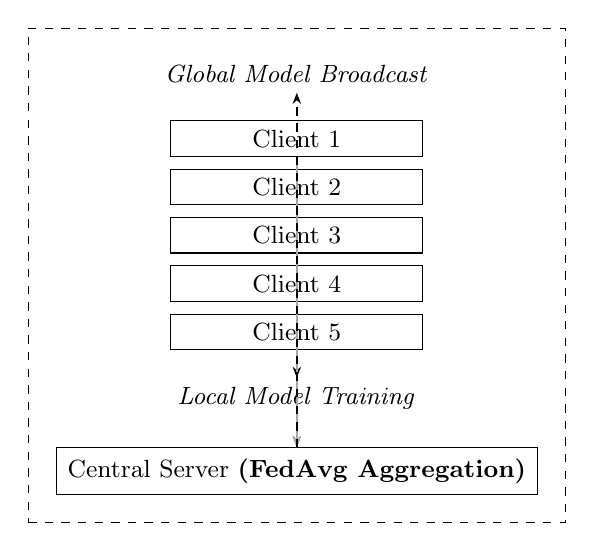
\begin{tikzpicture}[
    node distance=0.4cm,
    every node/.style={font=\small},
    client/.style={
        draw, rectangle,
        minimum width=3.2cm,
        minimum height=0.45cm,
        align=center,
        inner sep=3pt
    },
    server/.style={
        draw, rectangle,
        minimum width=4.5cm,
        minimum height=0.55cm,
        align=center,
        inner sep=4pt
    },
    arrow/.style={-{Stealth[length=4pt]}, thick}
]

%% ── Client nodes ──────────────────────────────────────
\node[client] (c1) {Client 1};
\node[client, below=0.15cm of c1] (c2) {Client 2};
\node[client, below=0.15cm of c2] (c3) {Client 3};
\node[client, below=0.15cm of c3] (c4) {Client 4};
\node[client, below=0.15cm of c4] (c5) {Client 5};

%% ── Downward arrow + label (Local Training) ──────────
\node[below=0.35cm of c5, align=center] (lt_label)
    {\textit{Local Model Training}};
\draw[arrow] (c5.south) -- (lt_label.north);

%% ── Central Server ────────────────────────────────────
\node[server, below=0.35cm of lt_label] (server)
    {Central Server \textbf{(FedAvg Aggregation)}};

%% ── Arrows from clients to server ────────────────────
\foreach \c in {c1,c2,c3,c4,c5}{
    \draw[arrow, gray!70] (\c.south)
        .. controls +(0,-0.2) and +(0,0.2) ..
        (server.north);
}

%% ── Global Model Update arrow (server back to clients)─
\node[above=0.35cm of c1, align=center] (gm_label)
    {\textit{Global Model Broadcast}};
\draw[arrow, dashed] (server.north)
    .. controls +(0,1.5) and +(0,-0.2) ..
    (gm_label.south);

%% ── Outer bounding box ────────────────────────────────
\begin{scope}[on background layer]
    \node[
        draw,
        rectangle,
        dashed,
        inner sep=10pt,
        fit=(gm_label)(c1)(c2)(c3)(c4)(c5)(lt_label)(server)
    ] {};
\end{scope}

\end{tikzpicture}
\caption{Proposed Federated Learning IDS architecture with multiple clients
and a central aggregation server.}
\label{fig:fl_architecture}
\end{figure}

Figure~\ref{fig:fl_architecture} illustrates the proposed FL-IDS architecture. The system follows a horizontal federated learning setup with five clients and a central aggregation server.

We chose five clients as a starting point to maintain a balance between simplicity and representativeness. Increasing the number of clients is certainly possible, but for a baseline study, this setup allows clearer interpretation of results.

\subsection{Stratified IID Partitioning Strategy}

The dataset is partitioned using a stratified IID approach. First, HIKARI-2021 is divided into six class-specific subsets. Each subset is then shuffled independently to remove ordering effects. Finally, each class is split equally across five clients.

This ensures that each client receives a balanced representation of all classes:
\begin{equation}
    \forall k, j: \quad |\mathcal{D}_k| = |\mathcal{D}_j| \;\text{and}\; P(y|\mathcal{D}_k) \approx P(y|\mathcal{D}_j)
\end{equation}

In practice, this creates a clean baseline for evaluation. While real-world data is rarely IID, starting with this setup allows us to isolate other factors before introducing additional complexity.

\subsection{Local Model Architecture}

Each client uses a simple feed-forward neural network. The architecture is intentionally kept straightforward to ensure reproducibility.

We include batch normalization to stabilize training and dropout ($p = 0.3$) to reduce overfitting. In our experiments, simpler models often generalize better in federated settings compared to overly complex architectures.

\begin{table}[h]
\centering
\caption{Local Client DNN Architecture}
\label{tab:dnn_arch}
\begin{tabular}{llll}
\hline
\textbf{Layer} & \textbf{Type}   & \textbf{Units/Rate} & \textbf{Activation} \\
\hline
1 & Input       & $d$ & ---     \\
2 & Dense       & 256 & ReLU    \\
3 & Batch Norm  & --- & ---     \\
4 & Dropout     & 0.3 & ---     \\
5 & Dense       & 128 & ReLU    \\
6 & Batch Norm  & --- & ---     \\
7 & Dense       & 64  & ReLU    \\
8 & Output      & 6   & Softmax \\
\hline
\end{tabular}
\end{table}

\subsection{Training Algorithm}

The training process follows the standard FL procedure described in~\cite{mcmahan2017}. Each client trains locally for $E$ epochs and shares only model updates with the server.

One key point to emphasize is that raw data never leaves the client. This is central to the privacy advantages of federated learning.

\subsection{Evaluation Metrics}

We evaluate performance using accuracy, precision, recall, and F1-score. Among these, macro-averaged F1 is the most informative metric for this dataset.

Since HIKARI-2021 is imbalanced, relying only on accuracy can be misleading. Macro-F1 ensures that minority attack classes are treated equally, which is important from a security perspective.


\section{Expected Performance Analysis}
\label{sec:performance}

\subsection{Projected Metrics}

Table~\ref{tab:projected_metrics} presents expected performance ranges based on similar studies~\cite{sun2023,liu2023,gao2023}. These values should be treated as estimates rather than exact predictions, and actual results may vary depending on implementation details and hyperparameter choices.

\begin{table}[h]
\centering
\caption{Projected FL-IDS Performance on HIKARI-2021 (IID Setting)}
\label{tab:projected_metrics}
\begin{tabular}{llll}
\hline
\textbf{Metric}         & \textbf{Min. Expected} & \textbf{Projected Range} & \textbf{Target} \\
\hline
Accuracy                & 88\%  & 92--95\%  & $>$95\% \\
Precision (macro)       & 84\%  & 89--93\%  & $>$90\% \\
Recall (macro)          & 82\%  & 88--92\%  & $>$90\% \\
F1-score (macro)        & 83\%  & 88--93\%  & $>$90\% \\
\hline
\end{tabular}
\end{table}

\subsection{Convergence Analysis}

Under IID conditions, FedAvg typically converges smoothly. Based on prior studies~\cite{mcmahan2017,li2022}, we expect convergence within 10--15 communication rounds for this setup.

Non-IID scenarios, however, are likely to slow convergence and introduce instability. This is one of the key motivations for future work on FedProx and related methods.

\subsection{Per-Class Analysis}

We expect higher performance for majority classes (Benign, Background) and lower performance for rare attack types such as Bruteforce-XML and XMRIGCC. This imbalance remains a challenge and may require techniques such as oversampling, class-weighted loss, or focal loss in follow-up studies.

\subsection{Communication Overhead}

Federated learning reduces data transfer compared to centralized training, but model updates still incur communication cost. Compression and hierarchical aggregation are practical directions to address this, as explored in Theme 3 of our review.


\section{Research Gap Analysis and Future Directions}
\label{sec:gaps}

\subsection{Systematic Gap Identification}

Our review highlights several important gaps. The most significant one is the absence of FL-based studies on HIKARI-2021, a dataset that is specifically designed for modern encrypted enterprise environments.

We also found that many studies rely on outdated datasets and do not consider encrypted traffic. These limitations reduce their relevance in real-world deployments. Non-IID settings remain underexplored, and privacy mechanisms such as differential privacy are rarely combined with practical IDS evaluation.

\subsection{Future Research Roadmap}

We outline five key directions for future work:

\textbf{Phase 1 --- Non-IID Experiments.} Evaluate performance under realistic data distributions using label-skew and device-based partitioning.

\textbf{Phase 2 --- Differential Privacy.} Study the tradeoff between privacy budget $\epsilon$ and detection accuracy on HIKARI-2021.

\textbf{Phase 3 --- Secure Aggregation.} Improve robustness against model poisoning and inference attacks.

\textbf{Phase 4 --- Hierarchical FL.} Scale the system to larger numbers of clients using a two-tier aggregation structure.

\textbf{Phase 5 --- Real-Time Deployment.} Test the system in practical network environments with live traffic streams.


\section{Conclusion}
\label{sec:conclusion}

In this paper, we reviewed 20 recent FL-IDS studies and identified several key limitations in current research. The surveyed works cover a range of approaches, from IoT-focused FL to privacy-enhanced and hierarchical architectures, and they collectively demonstrate that federated learning is a viable approach for intrusion detection.

The most important finding is that modern datasets like HIKARI-2021 remain underutilized in FL-IDS research, despite being better suited for real-world encrypted traffic scenarios. To address this, we proposed a federated learning framework based on FedAvg with stratified IID partitioning for six-class classification on HIKARI-2021.

We believe this work provides a useful foundation for future research in privacy-preserving intrusion detection, and the proposed roadmap offers concrete directions for extending the baseline toward more realistic and deployment-ready systems.

%% ── Acknowledgment ──────────────────────────────────────────────
\section*{Acknowledgment}
The authors gratefully acknowledge the guidance of Dr.\ Preeti Kathiria and the facilities provided by the Department of Computer Engineering, Institute of Technology, Nirma University, Ahmedabad, Gujarat, India.

%% ── References ─────────────────────────────────────────────────
\bibliographystyle{IEEEtran}
\bibliography{references}

\end{document}
